%%% maw.tex
%% \section{Minimal Absent Words and Maximal Repeats}
\section{Minimal Rare Words and Maximal Repeats}
\label{sec:mrep}

%% We introduce a fundamental concept of maximal repeats of a string $S$, which is useful for realizing efficient enumeration of many kinds of unusual words. Then, we give a characterization of the set $\MRW(S)$ of minimal rare words of a string $S$.
%% 
We introduce classes of unusual words of a string $S$.
A string $w \in \Sigma^*$ is \textit{trivial} if $|w| = 1$, i.e., $w = c$ for some letter $c$ in $\Sigma$, and \textit{non-trivial} otherwise.
We can easily see that any non-tivial string $w$ has length two and has the form $w = aub$ for some letter $a, b \in \hat\Sigma$ and a possibly string $u \in \Sigma^*$. Throughout, we assume $|\Sigma(S)|\ge 2$ and consider only non-trivial unusual words.
Let $S = S[1..n] \in \Sigma^n$ be a string over alphabet $\Sigma$.
For convention, we assume virtual extended string $\hat S[0..n+1] = \# S\daller \in \hat\Sigma^{n+2}$ obtained from $S$ by prepending and appending endmarkers, where $S[0] = \#$ and $S[n+1] = \daller$.

%%%% 
\mysubsubsection{Maximal repeats}
%%%%
Maximal repeats of a string is a fundamental concepts in discovery of unusual words, and introduced as follows.  
A \textit{repeat} of $S$ is any substring $u \in \Sigma^+$ that occurs at least twice in $S$, that is, $u \in \Fac(S)$.
Let $u \in \Sigma+$ be any factor of $\hat S$. Since $\#, \daller \not\in \Sigma$, we see $u \in \Fac(S)$, namely, $u$ is contained in the content $S$.

\begin{definition}[maximal repeat]\rm 
A string $u \in \Sigma+$ is a \textit{maximal repeat} of $S$ if it satisfies the following conditions: 
\begin{enumerate*}[(1)]
\item $u$ is a factor of $S$, i.e., $u \in \Fac(S)$;  
\item there exist two start positions $p, q \in \Spos[S](u)\;(p\not= q)$ of $u$ such that
  \begin{enumerate*}[(i)]
  \item $u$ is \textit{left-branching} meaning that the preceding characters are mutually different, i.e., $S[p-1] \not= S[q-1]$, and
  \item $u$ is \textit{right-branching} meaning that the following characters are mutually different, i.e., $S[p+|u|] \not= S[q+|u|]$. 
  \end{enumerate*}
\end{enumerate*}
\end{definition}

In what follows, $\MR(S)$ denotes the set of all maximal repeats of a string $S$. By definition, any $w$ in $\MR(S)$ correctly occurs at least twice in $S$. 
For later use, we define the \textit{set of left characters} $\LSigma(u) \subseteq \Sigma\cup\set{\#}$ (resp.~\textit{right characters} $\RSigma[](u) \subseteq \Sigma\cup\set{\daller}$) of a factor $u \in \Fac(S)$ to be the sets of all characters $S[p-1] \in \hat\Sigma$ (resp.~$S[p+|u|] \in \hat\Sigma$) preceding (resp.~following) all positions $p\in \Spos(u)$ of $u$ in $\hat S$.
If it is clear from context, we write $\LSigma[](u)$ and $\RSigma[](u)$ by omitting subscript $\hat S$. 
Using this notation, we can redefine a maximal repeat of $S$ to be any nonempty string $u \in \Fac(S)$ with $|\LSigma(u)| \ge 2$ and $|\RSigma(u)| \ge 2$.


%%%
\mysubsubsection{Minimal rare words}
%%%% 
The class of \textit{minimal rare words} was introduced by Belazzougui and Cunial~\cite{belazzougui2015space:unusual}, whose abstracted the properties of unusual words with statistical surprise studied by Apostolico, Bock, Lonardi, and Xu~\cite{apostolico2000efficient}.

\begin{definition}[minimal rare word]\rm 
For every integer $k\ge 0$, a \textit{$k$-minimal rare word} ($k$-MRW) of a string $S$ is a non-trivial string $w$ that occurs in $S$ exactly $k$ times, and any proper factor occurs in $S$ less frequently (see \cite{belazzougui2015space:unusual}). That is, a $k$-MRW of $S$ is a string $w = a u b$ with $a, b\in \hat\Sigma$ and $u \in \Sigma^+$ such that
\begin{enumerate*}[(i)]
\item $\Occ(aub) = k$; and 
\item $\Occ(au) > k$ and $\Occ(ub) > k$. 
\end{enumerate*}
We denote by $\MRW_k(S)$ and $\MRW(S) = \bigcup_{k\ge 0} \MRW_k(S)$ the sets of all $k$-MRWs and all MRWs of a string $S$, respectively.
\end{definition}

 %%%
Ilie and Smyth~\cite{ilie2011minimum} initiated the study of \textit{minimal unique substrings} (MUSs) of a string $S$, studied by Ilie and Smyth~\cite{ilie2011minimum}, is a non-trivial string $w$ that has unique occurrence in $S$, and any proper factor has more than one occurrences in $S$. 
That is, a MUS of $S$ is a string $w = a u b$ with $a, b\in \hat\Sigma$ and $u \in \Sigma^+$ such that
\begin{enumerate*}[(i)]
\item $\Occ(w) = 1$; and 
\item $\Occ(au) \ge 2$ and $\Occ(ub) \ge 2$. 
\end{enumerate*}
We denote by $\MAW(S)$ and $\MUS(S)$ the sets of all MAWs and all MUSs of a string $S$, respectively. 


As an example, the string $S = \texttt{aabaababb}$ has the following five maximal repeats $\tt \eps, a, aaba, ab$, and $\tt b$.
For instance, the factor $bab$ of $S$ is a $1$-minimal rare words since if we put $a = \op{b}, b = \op{b}$, $u = \op{a}$ and $k = 1$, we can check if the condition 
$\Occ(aub)= \Occ(\op{bab})= 1 = k$, 
$\Occ(au) = \Occ(\op{ba}) = 2 \ge k+1$, and 
$\Occ(ub) = \Occ(\op{ab}) = 3 \ge k+1$ hold. 

% of the string $S = \texttt{aabaababb}$ are shown in \cref{fig:example:maw}. 


%% \mysubsubsection[]{Minimal rare words}
%% %%%% 
%% (MRW, for short) of a string $S$ are a class of unusual words, introduced by
%% Belazzougui and Cunial~\cite{belazzougui2015space:unusual}
%% %% Garcia, Pinho, Rodrigues, Bastos, and Ferreira~\cite{garcia2011minimal}.
%% A \textit{MRW} is a non-trivial string $w$ that does not occur in $S$, and any proper factor of $w$ occurs in $S$ as a substring (see \cite{garcia2011minimal}).
%% Precisely, a MRW of $S$ is a string $a u b$ with $a, b\in \hat\Sigma$ and $u \in \Sigma^+$ such that
%% \begin{enumerate*}[(i)]
%% \item $w \not\in \Fac(\hat S)$; and 
%% \item $au, ub \in \Fac(\hat S)$. 
%% \end{enumerate*}

%% \mysubsubsection[]{Minimal absent words}
%% %%%% 
%% %A \textit{minimal absent word} (MRW)
%% of a string $S$ are a class of unusual words, introduced by Garcia, Pinho, Rodrigues, Bastos, and Ferreira~\cite{garcia2011minimal}. A \textit{MRW} is a non-trivial string $w$ that does not occur in $S$, and any proper factor of $w$ occurs in $S$ as a substring (see \cite{garcia2011minimal}).
%% Precisely, a MRW of $S$ is a string $a u b$ with $a, b\in \hat\Sigma$ and $u \in \Sigma^+$ such that
%% \begin{enumerate*}[(i)]
%% \item $w \not\in \Fac(\hat S)$; and 
%% \item $au, ub \in \Fac(\hat S)$. 
%% \end{enumerate*}

%% As an example, the minimal absent words of the string $S = \texttt{aabaababb}$ are shown in \cref{fig:example:maw}. 

%%%%%%
%% \begin{algorithm}[t]
%% \centering  
%% %% 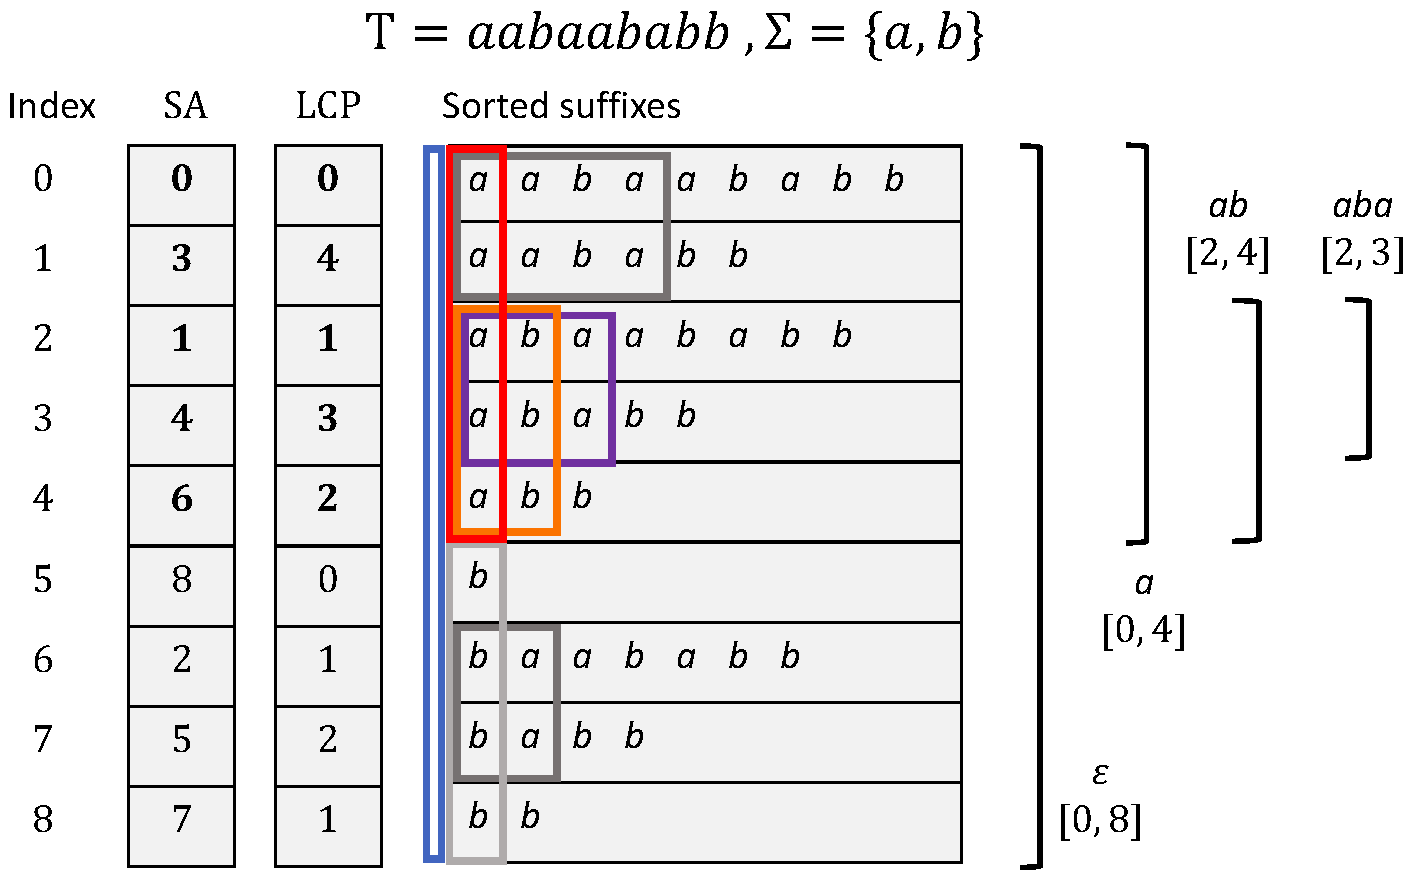
\includegraphics[width=0.60\textwidth]{fig/exp1/fig1.pdf}
%% \vspace{.5\baselineskip}
  %% \setlength{\interspacetitleruled}{0pt}%
%% \setlength{\algotitleheightrule}{0pt}%


%% %%%%%%
%% \begin{figure}[t]
%% \centering  
%% %% 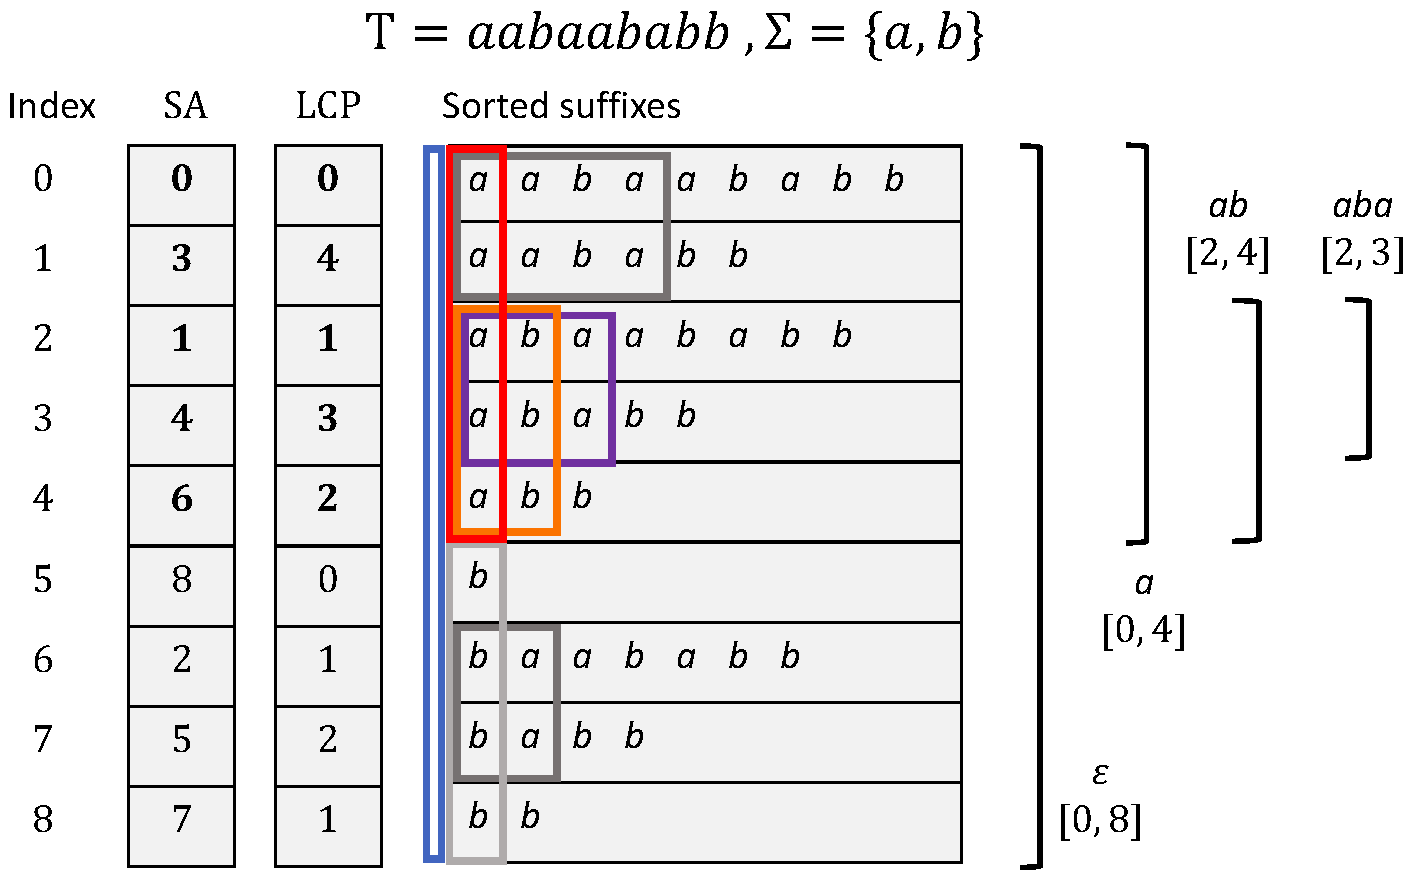
\includegraphics[width=0.60\textwidth]{fig/exp1/fig1.pdf}
%% \vspace{.5\baselineskip}
%% \caption{An example of minimal absent words of the string $S = \texttt{aabaababb}$. 
%% }\label{fig:example:maw}
%% \end{figure}
%% %%%%%%
%% %%%%%%%%%%%%%%%%%
%% \bgroup
%% {
%%   \setlength{\interspacetitleruled}{0pt}%
%%   \setlength{\algotitleheightrule}{0pt}%  
%%   \begin{algorithm}[h]
%%   %% \caption{Top-down MR-enumeration algorithm with \SA}\label{algo:maxrep:tdfw}
%%   \textbf{Procedure} \MRRec$(\tau_0 = ([L_0..R_0], \ell_0))$:\\
%%   %%\KwGiven{}
%%   %% \KwIn{The triple $\tau_0 = (L_0, R_0, \ell_0)$ for a right-branching substring $X$ of a string.}
%%   %% \KwOut{}
%%   \Begin{
%%       \textbf{output} $\tau_0$
%%       \Comment*{A maximal repeat is found}
%%       \For %(\CM{})
%%            {child $\tau = ([L..R], \ell)$ of the parent $([L_0..R_0], \ell_0)$}{
%%           \Comment{It is ensured that $R - L \ge 1$ and $\tau$ is right-branching}
%%           Decide if $\tau$ is left-branching by $\SA, \ISA$, and $S$ (\cref{lem:leftmaximal:character})\; 
%%           \If {$\tau$ is left-branching}{          
%%             \MRRec$(\tau)$\; 
%%           }
%%         }
%%   }
%%   \end{algorithm}
%% \egroup
%% %%%%%%%%%%%%%%%%%



%%% EOF
